\section{Theorie}
Der Begriff \enquote{Ultraschall} beschreibt den für Menschen nicht wahrnehmbaren Schall in einem Frequenzbereich von $\{\SI{20}{\kilo\hertz},\SI{1}{\giga\hertz}\}$.
\begin{align*}
    \text{Infraschall}  \textrightarrow \text{Hörbarer Bereich}  \textrightarrow \text{Ultraschall}  \textrightarrow \text{Hyperschall} 
\end{align*} 
Schall weist einen longitudinalen Wellencharakter auf, der duch Brechung oder Reflexion nachgewisen werden kann. Entsprechend lässt dieser sich also darstellen als
\begin{equation*}
    p(x,t) =  p_0 + \nu_0 Z \text{cos} (\omega t - kx).
\end{equation*}
Die Ausbreitung der Welle hängt von der sogenannten akustischen Impedanz $Z=c\cdot\rho$ ab, welche selbst ein Produkt der
Schallgeschwindigkeit $c$ und der Dichte $\rho$ des entsprechenden Mediums ist. Die Schallgeschwindkeit wiederum variiert bei verschieden Aggregatzuständen des verwendet Mediums
und wird bei Flüssigkeiten mit einer Kompressibilität $\kappa$ zu
\begin{equation*}
    c_{FL}=\sqrt{\frac{1}{\kappa \cdot \rho}}.
\end{equation*}
Fast Analog folgt der Zusammenhang bei Festkörpern der maßgeblich durch die nun zusätzliche Schubspannung dominiert wird und zudem stark richungsabhängig ist.
Diese Spannung lässt zusätzlich transversale Wellen zu und anstelle der reziproken Kompressibilität findet sich hier das Elastizitätsmodul $E$.
\begin{equation*}
    c_{FE}=\sqrt{\frac{E}{\rho}}
\end{equation*}
Die Bewegung von Schall verlangt ein Medium, wobei die Intensität aber exponentiell abfällt.
Der maßgebende Faktor dafür ist der Absorptionskoeffizient $\alpha$ und die ursprüglich einfallende Schallamplitude $I_0$.
\begin{equation}
    \label{eq:dummsumm}
    I(x)=I_0 \cdot e^{-\alpha x}
\end{equation}
Verschiedene Messungen von Absorptionskoeffizienten %maybe eine tabllle oder os refefn
zeigen, dass Luft eine äußerst hohe Absorption aufweist was sich nicht als nützlich in manchen Anwendungen erweist.
Des weiteren wird einfallender Schall auch bei ungewollten Grenzflächen mit einem Reflexionkoeffizienten $R$ reflektiert was anschließende Messungen erschwert.
Da die Intensität zu jedem Zeitpunkt erhalten bleiben muss findet sich der Transmissionskoeffizient der den transmittierten Anteil beschreibt.
Beide Koeffizienten müssen also in Summe $T+R=1$ geben um Verluste auszuschließen.
Die Reflexion wird durch die verschiedenen akustischen Impedanzen der verschieden Medien gebildet und lautet
\begin{equation*}
    R= \left( \frac{Z_1 - Z_2}{Z_1 + Z_2}\right)^2.
\end{equation*}
Um Schall mit solch hohen Frequenzen zu erzeugen, wird das Resultat des \enquote{piezo-elektrische Effekt} genutzt.
Dieser Effekt beschreibt das Wirken eines Piezokristalls in einem extern angelegtem elektrischen Feld. Die passenden Ausrichtung der polaren Achse des Kristalls zur Richtung des Felds 
lässt beispielsweise Quarz schwingen und somit Ultraschallwellen mit hoher Intensität abstrahlen wenn Resonanz zu beobachten ist.  
Umkehren lässt sich dieser Effekt, indem der Kristall Schallwellen ausgesetzt wird und so ein eigenes, später messbares, elektrisches Feld erzeugt. 
\\
\newline
In der Anwendung bieten sich besonders zwei Verfahren an um beispielsweise Informationen über Werkstoffe oder den Körper zu bekommen, ohne dabei 
die Medien zu zerstören oder zu deformieren.
\\
\newline
\begin{figure}
\begin{minipage}{0.5\textwidth}
\begin{description}
    \item [Durschallungs-Verfahren:] Dieser zweitelige Aufbau ist aufgeteilt in eine Sonde und einen Empfänger, welcher unter das Medium gelegt werden muss.
    Somit werden Fehlstellen durch abgeschwächte Intensitäten bemerkbar. \\
    \item [Impuls-Echo-Verfahren:] In diesem Fall fungiert der Sender zeitgleich als Empfänger. Es ist also nicht mehr nötig, unter das Medium reichen zu müssen was die Anwendung 
    erleichtert und handlicher macht. Außerdem gibt die Laufzeit $\Delta t$ des Schall, mit bekannter Schallgeschwindigkeit im zu durchstrahlenden Medium, 
    Aufschluss über die Entfernung der Fehlstelle
    \begin{equation}
        \label{eqn:WegvonSchallDurchEinMediumMitSchallgeschwindkeitCUndLaufzeitDeltaTWoebiDasBestimmtAuchAlsLichgeschwindgeitGesehenwerdenkannwennmankeineahnunghatundnichtdenkontextcheckt.}
        s = \frac{1}{2}c \Delta t.
    \end{equation}
\end{description}
\end{minipage}
\hfill
\begin{minipage}{0.4\textwidth}
    \centering
    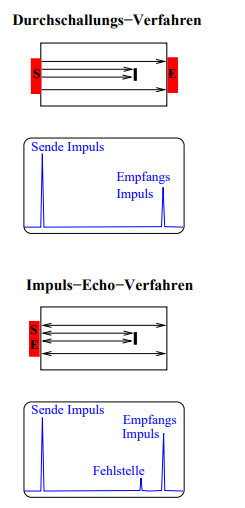
\includegraphics[width=0.7\textwidth]{Bilder/stuff.png}
    \captionsetup{justification=centering}
    \captionof{figure}{Schematische Darstellung der \\ zwei oben benannten Methoden. \cite{skript}}
    \label{fig:fig:fig:fig}
\end{minipage}
\end{figure}